\section{Assignment Three}\index{Assignment_Three}
\begin{enumerate}
\item
Check and verify the following:
\begin{enumerate}
\item
If $\bm M=\bm I-\bm u\bm v\trans$, then \[\bm M^{-1}=\bm I+\frac{\bm u\bm v\trans}{1-\bm v\trans\bm u}.\qquad(\bm v\trans\bm u\ne1)\]
\item
If $\bm M=\bm A-\bm u\bm v\trans$, then \[\bm M^{-1}=\bm A^{-1}+\frac{\bm A^{-1}\bm u\bm v\trans\bm A^{-1}}{1-\bm v\trans\bm A^{-1}\bm u}.\qquad(\bm v\trans\bm A^{-1}\bm u\ne1)\]
\item
If $\bm M=\bm I-\bm U\bm V$, where $\bm U\in\mathbb{R}^{n\x m},\bm V\in\mathbb{R}^{m\x n}$, then \[\bm M^{-1}=\bm I_n+\bm U(\bm I_m-\bm V\bm U)^{-1}\bm V.\]
\item
If $\bm M=\bm I-\bm U\bm W^{-1}\bm V$, where $\bm W\in\mathbb{R}^{m\x m},\bm U\in\mathbb{R}^{n\x m},\bm V\in\mathbb{R}^{m\x n}$, then \[\bm M^{-1}=\bm A^{-1}+\bm A^{-1}\bm U(\bm W-\bm V\bm A^{-1}\bm U)^{-1}\bm V\bm A^{-1}.\]
\end{enumerate}
\item
If $\bm A=\bm A\trans$ and $\bm B=\bm B\trans$, which of these matrices are certainly \textit{symmetric}?
\begin{enumerate}
\item
$\bm A^2-\bm B^2$
\item
$(\bm A+\bm B)(\bm A-\bm B)$
\item
$\bm{ABA}$
\item
$\bm{ABAB}$
\end{enumerate}
\item
Strat from LDU decomposition, show that each $n\x n$ matrix $\bm A$ can be factorized into a \textit{triangular} matrix times a \textit{symmetric} matrix.
\item
Let
\[
\bm A=\begin{bmatrix}
5&3\\3&2
\end{bmatrix},\quad\bm B=\begin{bmatrix}
6&2\\2&4
\end{bmatrix},\quad\bm C=\begin{bmatrix}
4&-2\\-6&3
\end{bmatrix}
\]
solve each of the following matrix equations:
\begin{enumerate}
\item
$\bm{Ax}+\bm B=\bm C$
\item
$\bm{XA}+\bm B=\bm C$
\item
$\bm{AX}+\bm B=\bm X$
\item
$\bm{XA}+\bm C=\bm X$
\end{enumerate}
\item
Let $\bm U$ and $\bm R$ be $n\x n$ upper triangular matrices and $\bm T=\bm{UR}$, show that $\bm T$ is also \textit{upper triangular} and that $t_{jj}=u_{jj}r_{jj},j=1,\dots,n.$
\item
Consider the graph
\begin{figure}[H]
\centering
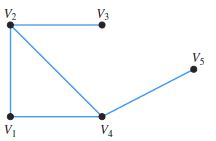
\includegraphics{week2/adj}
\end{figure}
\begin{enumerate}
\item
Determine the adjacency matrix $\bm A$ of the graph.
\item
Compute $\bm A^2$. What do the entries in the first row of $\bm A^2$ tell you about walks of length $2$ that start from $V_1$?
\item
Compute $\bm A^3$. How many walks of length $3$
are there from $V_2$ to $V_3$? How many walks of
length \textit{less than} or \textit{equal} to $3$ are there from $\bm V_2$ to $\bm V_4$?
\end{enumerate}
\end{enumerate}